\documentclass{report}

% PACKAGES
\usepackage[margin=1.00in]{geometry}
\usepackage[pdftex]{graphicx}
\usepackage{indentfirst}

\usepackage{Sweave}
\begin{document}
\Sconcordance{concordance:upstat_report.tex:upstat_report.Rnw:%
1 12 1 1 0 23 1 1 25 45 1 1 23 1 2 26 1 1 22 1 2 24 1 1 91 1 23 1 2 24 %
1 1 15 1 2 15 1 1 10 1 2 9 1 1 88 1 2 29 1}

\begin{titlepage}

\begin{center}

~\\[4cm]

\textsc{\Large Culver Road and East Main Street Intersection}\\[1.5cm]
\textsc{\huge Traffic Analysis Report}\\[8.5cm]



\vfill

{ March 20, 2015}

\end{center}
\end{titlepage}

\noindent
\section*{Introduction}

%This subsection should include a diagram of the interesction and some statistics
%about the interection. This should include information about the traffic flow
%rate (volume), the LOC classification, and some general information that is
%useful to the DOT.



\noindent
\section*{Data Analysis}

To assess the traffic conditions at the Culver Road and East Main Street
intersection, we performed analyses to examine trends and patterns in the traffic
observed, as well as methods for predicting traffic congestions based on time of
day, day of the week, and the weather conditions present.


\subsection*{Trend and Pattern Analysis}

To examine the general trend in the metrics we were provided, we performed linear
and multivariate regression. These techniques allows us to approximate the traffic
volume and delay. As shown in Figure \ref{trends}. Lorem ipsum dolor sit amet,
consectetur adipiscing elit. Donec vitae nunc quis sem cursus luctus in at est.
Etiam at augue ac libero interdum euismod non nec sem. Aliquam erat volutpat.
Phasellus auctor urna purus, ac rutrum eros fermentum ut. Lorem ipsum dolor sit
amet, consectetur adipiscing elit.

\begin{figure}[h]
\centering
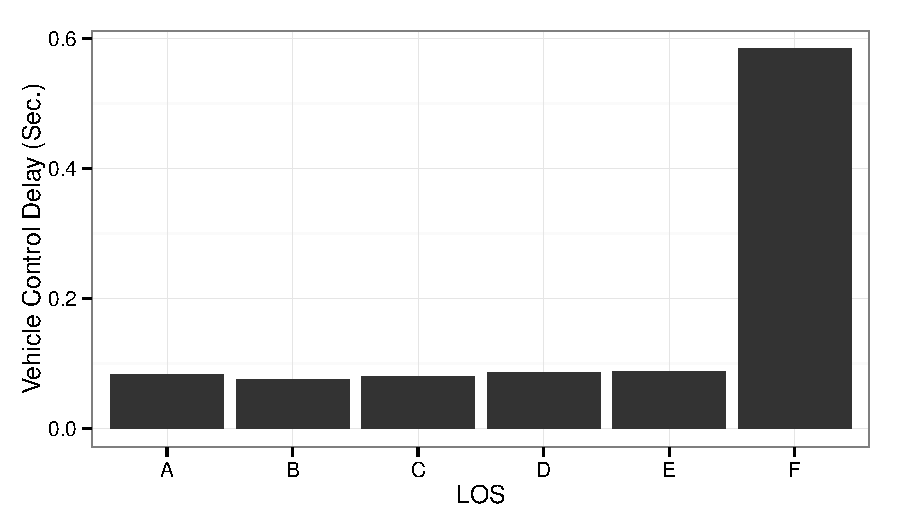
\includegraphics{upstat_report-002}
\caption{The median delay and volume is increasing over time. Lorem ipsum dolor
sit amet, consectetur adipiscing elit. Donec vitae nunc quis sem cursus luctus
in at est. Etiam at augue ac libero interdum euismod non nec sem. Aliquam erat
volutpat. Phasellus auctor urna purus, ac rutrum eros fermentum ut. Lorem ipsum
dolor sit amet, consectetur adipiscing elit.}
\label{trends}
\end{figure}

\subsection*{Bayesian Analysis}
\subsection*{Weather Analysis}

\noindent\section*{Recommendations}

Nuke Rochester.

\noindent
\section*{Cited Literature}

Leviticus.

\end{document}
